% Options for packages loaded elsewhere
\PassOptionsToPackage{unicode}{hyperref}
\PassOptionsToPackage{hyphens}{url}
%
\documentclass[
  12pt,
]{book}
\usepackage{amsmath,amssymb}
\usepackage{lmodern}
\usepackage{setspace}
\usepackage{ifxetex,ifluatex}
\ifnum 0\ifxetex 1\fi\ifluatex 1\fi=0 % if pdftex
  \usepackage[T1]{fontenc}
  \usepackage[utf8]{inputenc}
  \usepackage{textcomp} % provide euro and other symbols
\else % if luatex or xetex
  \usepackage{unicode-math}
  \defaultfontfeatures{Scale=MatchLowercase}
  \defaultfontfeatures[\rmfamily]{Ligatures=TeX,Scale=1}
\fi
% Use upquote if available, for straight quotes in verbatim environments
\IfFileExists{upquote.sty}{\usepackage{upquote}}{}
\IfFileExists{microtype.sty}{% use microtype if available
  \usepackage[]{microtype}
  \UseMicrotypeSet[protrusion]{basicmath} % disable protrusion for tt fonts
}{}
\makeatletter
\@ifundefined{KOMAClassName}{% if non-KOMA class
  \IfFileExists{parskip.sty}{%
    \usepackage{parskip}
  }{% else
    \setlength{\parindent}{0pt}
    \setlength{\parskip}{6pt plus 2pt minus 1pt}}
}{% if KOMA class
  \KOMAoptions{parskip=half}}
\makeatother
\usepackage{xcolor}
\IfFileExists{xurl.sty}{\usepackage{xurl}}{} % add URL line breaks if available
\IfFileExists{bookmark.sty}{\usepackage{bookmark}}{\usepackage{hyperref}}
\hypersetup{
  pdftitle={İstatistiksel Testler},
  pdfauthor={Mustafa Murat ARAT},
  hidelinks,
  pdfcreator={LaTeX via pandoc}}
\urlstyle{same} % disable monospaced font for URLs
\usepackage{color}
\usepackage{fancyvrb}
\newcommand{\VerbBar}{|}
\newcommand{\VERB}{\Verb[commandchars=\\\{\}]}
\DefineVerbatimEnvironment{Highlighting}{Verbatim}{commandchars=\\\{\}}
% Add ',fontsize=\small' for more characters per line
\usepackage{framed}
\definecolor{shadecolor}{RGB}{248,248,248}
\newenvironment{Shaded}{\begin{snugshade}}{\end{snugshade}}
\newcommand{\AlertTok}[1]{\textcolor[rgb]{0.94,0.16,0.16}{#1}}
\newcommand{\AnnotationTok}[1]{\textcolor[rgb]{0.56,0.35,0.01}{\textbf{\textit{#1}}}}
\newcommand{\AttributeTok}[1]{\textcolor[rgb]{0.77,0.63,0.00}{#1}}
\newcommand{\BaseNTok}[1]{\textcolor[rgb]{0.00,0.00,0.81}{#1}}
\newcommand{\BuiltInTok}[1]{#1}
\newcommand{\CharTok}[1]{\textcolor[rgb]{0.31,0.60,0.02}{#1}}
\newcommand{\CommentTok}[1]{\textcolor[rgb]{0.56,0.35,0.01}{\textit{#1}}}
\newcommand{\CommentVarTok}[1]{\textcolor[rgb]{0.56,0.35,0.01}{\textbf{\textit{#1}}}}
\newcommand{\ConstantTok}[1]{\textcolor[rgb]{0.00,0.00,0.00}{#1}}
\newcommand{\ControlFlowTok}[1]{\textcolor[rgb]{0.13,0.29,0.53}{\textbf{#1}}}
\newcommand{\DataTypeTok}[1]{\textcolor[rgb]{0.13,0.29,0.53}{#1}}
\newcommand{\DecValTok}[1]{\textcolor[rgb]{0.00,0.00,0.81}{#1}}
\newcommand{\DocumentationTok}[1]{\textcolor[rgb]{0.56,0.35,0.01}{\textbf{\textit{#1}}}}
\newcommand{\ErrorTok}[1]{\textcolor[rgb]{0.64,0.00,0.00}{\textbf{#1}}}
\newcommand{\ExtensionTok}[1]{#1}
\newcommand{\FloatTok}[1]{\textcolor[rgb]{0.00,0.00,0.81}{#1}}
\newcommand{\FunctionTok}[1]{\textcolor[rgb]{0.00,0.00,0.00}{#1}}
\newcommand{\ImportTok}[1]{#1}
\newcommand{\InformationTok}[1]{\textcolor[rgb]{0.56,0.35,0.01}{\textbf{\textit{#1}}}}
\newcommand{\KeywordTok}[1]{\textcolor[rgb]{0.13,0.29,0.53}{\textbf{#1}}}
\newcommand{\NormalTok}[1]{#1}
\newcommand{\OperatorTok}[1]{\textcolor[rgb]{0.81,0.36,0.00}{\textbf{#1}}}
\newcommand{\OtherTok}[1]{\textcolor[rgb]{0.56,0.35,0.01}{#1}}
\newcommand{\PreprocessorTok}[1]{\textcolor[rgb]{0.56,0.35,0.01}{\textit{#1}}}
\newcommand{\RegionMarkerTok}[1]{#1}
\newcommand{\SpecialCharTok}[1]{\textcolor[rgb]{0.00,0.00,0.00}{#1}}
\newcommand{\SpecialStringTok}[1]{\textcolor[rgb]{0.31,0.60,0.02}{#1}}
\newcommand{\StringTok}[1]{\textcolor[rgb]{0.31,0.60,0.02}{#1}}
\newcommand{\VariableTok}[1]{\textcolor[rgb]{0.00,0.00,0.00}{#1}}
\newcommand{\VerbatimStringTok}[1]{\textcolor[rgb]{0.31,0.60,0.02}{#1}}
\newcommand{\WarningTok}[1]{\textcolor[rgb]{0.56,0.35,0.01}{\textbf{\textit{#1}}}}
\usepackage{longtable,booktabs,array}
\usepackage{calc} % for calculating minipage widths
% Correct order of tables after \paragraph or \subparagraph
\usepackage{etoolbox}
\makeatletter
\patchcmd\longtable{\par}{\if@noskipsec\mbox{}\fi\par}{}{}
\makeatother
% Allow footnotes in longtable head/foot
\IfFileExists{footnotehyper.sty}{\usepackage{footnotehyper}}{\usepackage{footnote}}
\makesavenoteenv{longtable}
\usepackage{graphicx}
\makeatletter
\def\maxwidth{\ifdim\Gin@nat@width>\linewidth\linewidth\else\Gin@nat@width\fi}
\def\maxheight{\ifdim\Gin@nat@height>\textheight\textheight\else\Gin@nat@height\fi}
\makeatother
% Scale images if necessary, so that they will not overflow the page
% margins by default, and it is still possible to overwrite the defaults
% using explicit options in \includegraphics[width, height, ...]{}
\setkeys{Gin}{width=\maxwidth,height=\maxheight,keepaspectratio}
% Set default figure placement to htbp
\makeatletter
\def\fps@figure{htbp}
\makeatother
\setlength{\emergencystretch}{3em} % prevent overfull lines
\providecommand{\tightlist}{%
  \setlength{\itemsep}{0pt}\setlength{\parskip}{0pt}}
\setcounter{secnumdepth}{5}
\usepackage{booktabs}
\AtBeginDocument{\renewcommand{\chaptername}{Bölüm}}
\ifluatex
  \usepackage{selnolig}  % disable illegal ligatures
\fi
\usepackage[]{natbib}
\bibliographystyle{apalike}

\title{İstatistiksel Testler}
\author{Mustafa Murat ARAT}
\date{2021-02-22}

\begin{document}
\maketitle

{
\setcounter{tocdepth}{3}
\tableofcontents
}
\setstretch{1.5}
\hypertarget{uxf6nsuxf6z}{%
\chapter*{Önsöz}\label{uxf6nsuxf6z}}
\addcontentsline{toc}{chapter}{Önsöz}

This is the very first part of the book.

bookdown::render\_book(`index.Rmd', `bookdown::pdf\_book')
bookdown::render\_book(`index.Rmd', `bookdown::epub\_book')

\hypertarget{introduction}{%
\chapter{Giriş}\label{introduction}}

BLABLABLA

\hypertarget{statisticalterms}{%
\chapter{İstatistiksel Terimler}\label{statisticalterms}}

\hypertarget{kullanux131lan-semboller}{%
\section{Kullanılan Semboller}\label{kullanux131lan-semboller}}

\(n\): gözlem sayısı (örneklem büyüklüğü)

\(K\): örneklem sayısı (her biri n elemana sahip)

\(\alpha\): anlamlılık düzeyi

\(\nu\): serbestlik derecesi

\(\sigma\): standart sapma (kitle)

\(s\): standart sapma (örneklem)

\(\mu\): kitle (popülasyon) ortalaması

\(\overline{x}\): örneklem ortalaması

\(\rho\): kitle (popülasyon) korelasyon katsayısı

\(r\): örneklem korelasyon katsayısı

\(Z\): standart normal sapma

\hypertarget{tests}{%
\chapter{Testler}\label{tests}}

\hypertarget{test-1---bir-popuxfclasyon-ortalamasux131-iuxe7in-z-testi-bilinen-varyans}{%
\section{Test 1 - Bir popülasyon ortalaması için Z testi (bilinen varyans)}\label{test-1---bir-popuxfclasyon-ortalamasux131-iuxe7in-z-testi-bilinen-varyans}}

\hypertarget{amauxe7}{%
\subsection{Amaç}\label{amauxe7}}

Popülasyon varyansı bilindiğinde bir varsayılan popülasyon ortalaması \(\mu_{0}\) ve bir örneklem ortalaması \(\overline{x}\) arasındaki anlamlığının araştırılması

\hypertarget{kux131sux131tlar}{%
\subsection{Kısıtlar}\label{kux131sux131tlar}}

1.Popülasyon varyansı \(\sigma^{2}\)'nin bilinmesi gereklidir. (\(\sigma^{2}\) bilinmiyorsa, bir popülasyon ortalaması için t testine bakınız.)
2. Popülasyon normal dağılıyorsa, test doğrudur. Normal dağılmıyorsa, test yine de yaklaşık bir sonuç verecektir.

\hypertarget{yuxf6ntem}{%
\subsection{Yöntem}\label{yuxf6ntem}}

Ortalaması \(\mu_{0}\) ve bilinen varyansı \(\sigma^{2}\) olan bir popülasyondan, \(n\) büyüklüğünde rastgele bir örneklem alınır ve örneklem ortalaması \(\overline{x}\) hesaplanır. Test istatistiği olan

\begin{equation}
Z = \frac{\overline{x} - \mu_{0}}{\sigma / \sqrt{n}}
\end{equation}

bir veya iki yönlü ve \(\alpha\) büyüklüğünde kritik bölgeye sahip standart normal dağılımla karşılaştırılabilir.

\hypertarget{uxf6rnek}{%
\subsection{Örnek}\label{uxf6rnek}}

Belirli bir kozmetik yelpazesi için, yüz pudrasının olduğu kutuları doldurmak için ortalama 4 gm ve standart sapma 1 gm olacak şekilde bir doldurma işlemi yapılmaktadır. Bir kalite kontrol müfettişi rastgele dokuz kutudan numune almaktadır ve her bir kutudaki tozu tartmaktadır. Ortalama toz ağırlığı 4,6 gramdır. Dolgu işlemi hakkında neler söylenebilir?

Aşırı ve az doldurma konusunda endişeliysek iki yönlü bir test kullanılabilir. Öte yandan, sadece kozmetik malzemenin fazla doldurulmasıyla ilgileniyorsak tek yönlü bir test uygundur.

\textbf{Sayısal Hesaplama}

\(\mu_{0} = 4.0\), \(n=9\), \(\overline{x} = 4.6\), \(\sigma = 1.0\), \(\alpha = 0.05\) (\(\%95\) güven düzeyine sahip)

\(Z = \dfrac{\overline{x} - \mu_{0}}{\sigma / \sqrt{n}} = \frac{4.6 - 4.0}{1.0 / \sqrt{9}} = \frac{0.6}{1/3} = 1.8\)

Eğer iki yönlü hipotez testi kullanmak isterseniz, kurmanız gereken hipotezler aşağıdaki gibidir:

\(H_{0}: \mu = \mu_{0},\,\,\, H_{1}: \mu \neq \mu_{0}\).

Bu durumda kabul bölgesi \(−1.96 < Z < 1.96\)'dır çünkü kritik değer \(Z_{\alpha/2} = Z_{0.025} = 1.96\).

\begin{Shaded}
\begin{Highlighting}[]
\FunctionTok{library}\NormalTok{(ggplot2)}
\FunctionTok{ggplot}\NormalTok{(}\ConstantTok{NULL}\NormalTok{, }\FunctionTok{aes}\NormalTok{(}\FunctionTok{c}\NormalTok{(}\SpecialCharTok{{-}}\DecValTok{3}\NormalTok{,}\DecValTok{1}\NormalTok{))) }\SpecialCharTok{+}
  \FunctionTok{geom\_area}\NormalTok{(}\AttributeTok{stat =} \StringTok{"function"}\NormalTok{, }\AttributeTok{fun =}\NormalTok{ dnorm, }\AttributeTok{fill =} \StringTok{"grey80"}\NormalTok{, }\AttributeTok{xlim =} \FunctionTok{c}\NormalTok{(}\SpecialCharTok{{-}}\DecValTok{3}\NormalTok{, }\SpecialCharTok{{-}}\FloatTok{1.96}\NormalTok{)) }\SpecialCharTok{+}
  \FunctionTok{geom\_area}\NormalTok{(}\AttributeTok{stat =} \StringTok{"function"}\NormalTok{, }\AttributeTok{fun =}\NormalTok{ dnorm, }\AttributeTok{fill =} \StringTok{"\#FAD623"}\NormalTok{, }\AttributeTok{xlim =} \FunctionTok{c}\NormalTok{(}\SpecialCharTok{{-}}\FloatTok{1.96}\NormalTok{, }\FloatTok{1.96}\NormalTok{)) }\SpecialCharTok{+}
  \FunctionTok{geom\_area}\NormalTok{(}\AttributeTok{stat =} \StringTok{"function"}\NormalTok{, }\AttributeTok{fun =}\NormalTok{ dnorm, }\AttributeTok{fill =} \StringTok{"grey80"}\NormalTok{, }\AttributeTok{xlim =} \FunctionTok{c}\NormalTok{(}\FloatTok{1.96}\NormalTok{, }\DecValTok{3}\NormalTok{)) }\SpecialCharTok{+}
  \FunctionTok{geom\_vline}\NormalTok{(}\AttributeTok{xintercept =} \DecValTok{0}\NormalTok{, }\AttributeTok{color =} \StringTok{"\#6C0606"}\NormalTok{, }\AttributeTok{linetype =} \StringTok{"dotted"}\NormalTok{) }\SpecialCharTok{+}
  \FunctionTok{geom\_vline}\NormalTok{(}\AttributeTok{xintercept =} \FloatTok{1.8}\NormalTok{, }\AttributeTok{color =} \StringTok{"\#000000"}\NormalTok{, }\AttributeTok{lwd=}\DecValTok{1}\NormalTok{, }\AttributeTok{linetype =} \StringTok{"dashed"}\NormalTok{) }\SpecialCharTok{+}
  \FunctionTok{labs}\NormalTok{(}\AttributeTok{x =} \StringTok{"z"}\NormalTok{, }\AttributeTok{y =} \StringTok{""}\NormalTok{) }\SpecialCharTok{+}
  \FunctionTok{scale\_y\_continuous}\NormalTok{(}\AttributeTok{breaks =} \ConstantTok{NULL}\NormalTok{) }\SpecialCharTok{+}
  \FunctionTok{scale\_x\_continuous}\NormalTok{(}\AttributeTok{breaks =} \FunctionTok{c}\NormalTok{(}\SpecialCharTok{{-}}\FloatTok{1.96}\NormalTok{, }\DecValTok{0}\NormalTok{, }\FloatTok{1.96}\NormalTok{))}\SpecialCharTok{+}
  \FunctionTok{annotate}\NormalTok{(}\StringTok{"label"}\NormalTok{, }\AttributeTok{x =} \DecValTok{0}\NormalTok{, }\AttributeTok{y =} \FloatTok{0.2}\NormalTok{, }\AttributeTok{label =} \StringTok{"KABUL BÖLGESİ"}\NormalTok{)}\SpecialCharTok{+}
  \FunctionTok{annotate}\NormalTok{(}\StringTok{"segment"}\NormalTok{, }\AttributeTok{x =} \FloatTok{2.3}\NormalTok{, }\AttributeTok{xend =} \FloatTok{2.65}\NormalTok{, }\AttributeTok{y =} \FloatTok{0.015}\NormalTok{, }\AttributeTok{yend =}\FloatTok{0.04}\NormalTok{,}
           \AttributeTok{colour =} \StringTok{"black"}\NormalTok{, }\AttributeTok{size =} \FloatTok{0.95}\NormalTok{, }\AttributeTok{arrow =} \FunctionTok{arrow}\NormalTok{(}\AttributeTok{type =} \StringTok{"closed"}\NormalTok{, }\AttributeTok{length =} \FunctionTok{unit}\NormalTok{(}\FloatTok{0.02}\NormalTok{, }\StringTok{"npc"}\NormalTok{))) }\SpecialCharTok{+}
  \FunctionTok{annotate}\NormalTok{(}\StringTok{"text"}\NormalTok{, }\AttributeTok{x=}\FloatTok{2.66}\NormalTok{, }\AttributeTok{y=}\FloatTok{0.048}\NormalTok{, }\AttributeTok{label=}\StringTok{\textquotesingle{}0.025\textquotesingle{}}\NormalTok{)}\SpecialCharTok{+}
  \FunctionTok{annotate}\NormalTok{(}\StringTok{"segment"}\NormalTok{, }\AttributeTok{x =} \SpecialCharTok{{-}}\FloatTok{2.3}\NormalTok{, }\AttributeTok{xend =} \SpecialCharTok{{-}}\FloatTok{2.65}\NormalTok{, }\AttributeTok{y =} \FloatTok{0.015}\NormalTok{, }\AttributeTok{yend =}\FloatTok{0.04}\NormalTok{,}
           \AttributeTok{colour =} \StringTok{"black"}\NormalTok{, }\AttributeTok{size =} \FloatTok{0.95}\NormalTok{, }\AttributeTok{arrow =} \FunctionTok{arrow}\NormalTok{(}\AttributeTok{type =} \StringTok{"closed"}\NormalTok{, }\AttributeTok{length =} \FunctionTok{unit}\NormalTok{(}\FloatTok{0.02}\NormalTok{, }\StringTok{"npc"}\NormalTok{))) }\SpecialCharTok{+}
  \FunctionTok{annotate}\NormalTok{(}\StringTok{"text"}\NormalTok{, }\AttributeTok{x=}\SpecialCharTok{{-}}\FloatTok{2.66}\NormalTok{, }\AttributeTok{y=}\FloatTok{0.048}\NormalTok{, }\AttributeTok{label=}\StringTok{\textquotesingle{}0.025\textquotesingle{}}\NormalTok{)}
\end{Highlighting}
\end{Shaded}

\begin{verbatim}
## Warning in grid.Call(C_textBounds, as.graphicsAnnot(x$label), x$x, x$y, :
## conversion failure on 'KABUL BÖLGESİ' in 'mbcsToSbcs': dot substituted for <c4>
\end{verbatim}

\begin{verbatim}
## Warning in grid.Call(C_textBounds, as.graphicsAnnot(x$label), x$x, x$y, :
## conversion failure on 'KABUL BÖLGESİ' in 'mbcsToSbcs': dot substituted for <b0>
\end{verbatim}

\begin{verbatim}
## Warning in grid.Call(C_textBounds, as.graphicsAnnot(x$label), x$x, x$y, :
## conversion failure on 'KABUL BÖLGESİ' in 'mbcsToSbcs': dot substituted for <c4>
\end{verbatim}

\begin{verbatim}
## Warning in grid.Call(C_textBounds, as.graphicsAnnot(x$label), x$x, x$y, :
## conversion failure on 'KABUL BÖLGESİ' in 'mbcsToSbcs': dot substituted for <b0>
\end{verbatim}

\begin{verbatim}
## Warning in grid.Call.graphics(C_text, as.graphicsAnnot(x$label), x$x, x$y, :
## conversion failure on 'KABUL BÖLGESİ' in 'mbcsToSbcs': dot substituted for <c4>
\end{verbatim}

\begin{verbatim}
## Warning in grid.Call.graphics(C_text, as.graphicsAnnot(x$label), x$x, x$y, :
## conversion failure on 'KABUL BÖLGESİ' in 'mbcsToSbcs': dot substituted for <b0>
\end{verbatim}

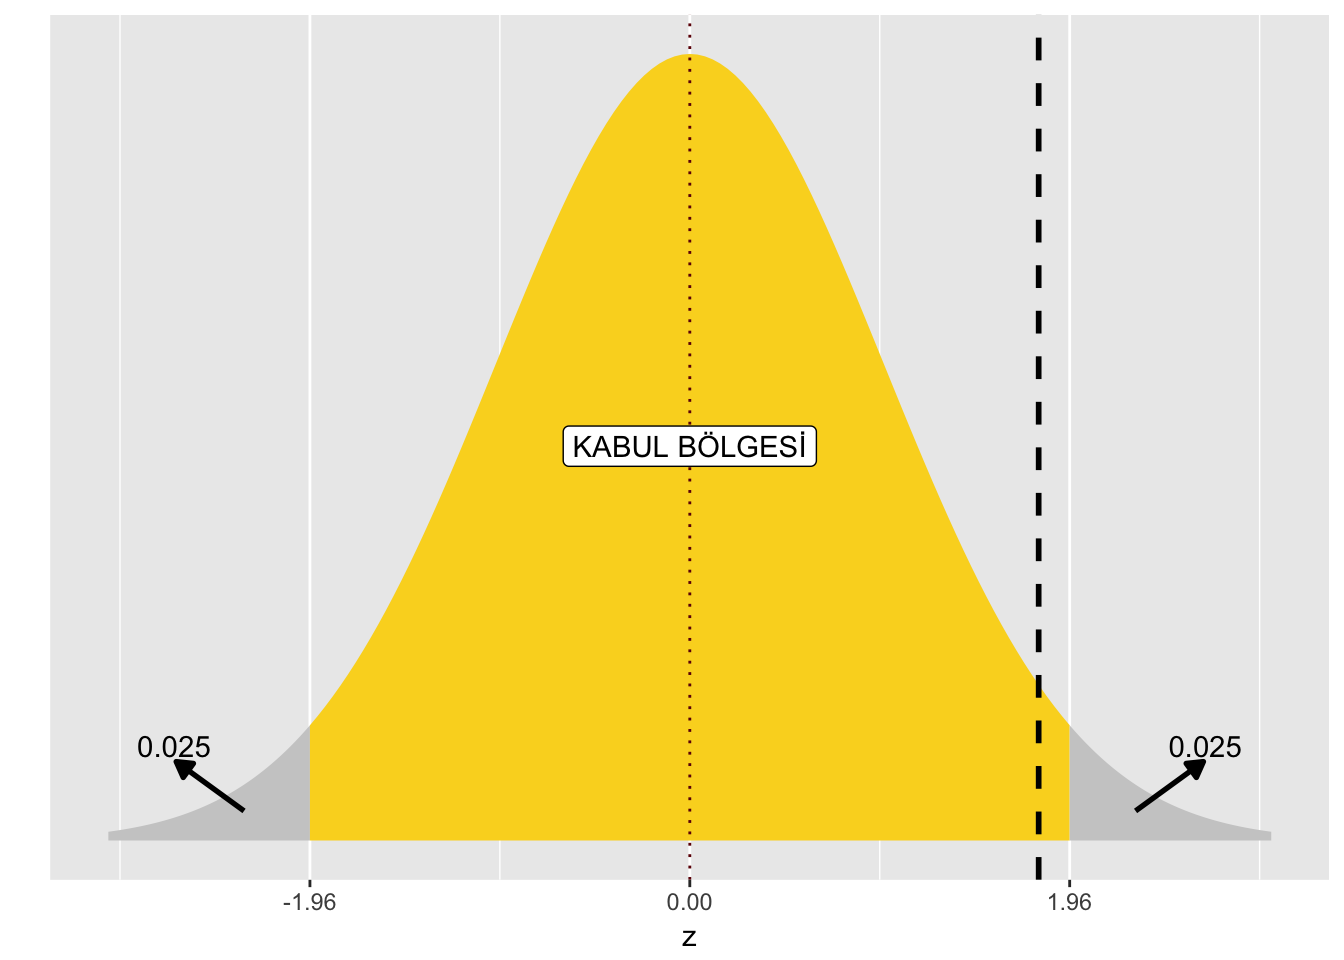
\includegraphics{03-Tests_files/figure-latex/unnamed-chunk-1-1.pdf}

Test istatistiği, taralı alan olan kabul bölgesine düstüğü için \(H_{0}\) boş hipotezini red edemezsiniz. Yani, bu numune (örneklem) için doldurma işleminin hedefte çalışmadığını öne sürmek için hiçbir neden yoktur.

Eğer tek yönlü hipotez testi kurmak isteseydiniz, kuracağınız hipotezler aşağıdaki gibidir:

\(H_{0}: \mu = \mu_{0},\,\,\, H_{1}: \mu > \mu_{0}\).

Bu durumda kabul bölgesi \(Z < 1.65\)'dır çünkü kritik değer \(Z_{\alpha} = Z_{0.05} = 1.65\)'tir.

\begin{Shaded}
\begin{Highlighting}[]
\FunctionTok{library}\NormalTok{(ggplot2)}
\FunctionTok{ggplot}\NormalTok{(}\ConstantTok{NULL}\NormalTok{, }\FunctionTok{aes}\NormalTok{(}\FunctionTok{c}\NormalTok{(}\SpecialCharTok{{-}}\DecValTok{3}\NormalTok{,}\DecValTok{1}\NormalTok{))) }\SpecialCharTok{+}
  \FunctionTok{geom\_area}\NormalTok{(}\AttributeTok{stat =} \StringTok{"function"}\NormalTok{, }\AttributeTok{fun =}\NormalTok{ dnorm, }\AttributeTok{fill =} \StringTok{"\#AB1616"}\NormalTok{, }\AttributeTok{xlim =} \FunctionTok{c}\NormalTok{(}\SpecialCharTok{{-}}\DecValTok{3}\NormalTok{, }\FloatTok{1.65}\NormalTok{)) }\SpecialCharTok{+}
  \FunctionTok{geom\_area}\NormalTok{(}\AttributeTok{stat =} \StringTok{"function"}\NormalTok{, }\AttributeTok{fun =}\NormalTok{ dnorm, }\AttributeTok{fill =} \StringTok{"grey80"}\NormalTok{, }\AttributeTok{xlim =} \FunctionTok{c}\NormalTok{(}\FloatTok{1.65}\NormalTok{, }\DecValTok{3}\NormalTok{)) }\SpecialCharTok{+}
  \FunctionTok{geom\_vline}\NormalTok{(}\AttributeTok{xintercept =} \DecValTok{0}\NormalTok{, }\AttributeTok{color =} \StringTok{"\#6C0606"}\NormalTok{, }\AttributeTok{linetype =} \StringTok{"dotted"}\NormalTok{) }\SpecialCharTok{+}
  \FunctionTok{geom\_vline}\NormalTok{(}\AttributeTok{xintercept =} \FloatTok{1.8}\NormalTok{, }\AttributeTok{color =} \StringTok{"\#000000"}\NormalTok{, }\AttributeTok{lwd=}\DecValTok{1}\NormalTok{, }\AttributeTok{linetype =} \StringTok{"dashed"}\NormalTok{) }\SpecialCharTok{+}
  \FunctionTok{labs}\NormalTok{(}\AttributeTok{x =} \StringTok{"z"}\NormalTok{, }\AttributeTok{y =} \StringTok{""}\NormalTok{) }\SpecialCharTok{+}
  \FunctionTok{scale\_y\_continuous}\NormalTok{(}\AttributeTok{breaks =} \ConstantTok{NULL}\NormalTok{) }\SpecialCharTok{+}
  \FunctionTok{scale\_x\_continuous}\NormalTok{(}\AttributeTok{breaks =} \FunctionTok{c}\NormalTok{(}\SpecialCharTok{{-}}\FloatTok{1.65}\NormalTok{, }\DecValTok{0}\NormalTok{, }\FloatTok{1.65}\NormalTok{))}\SpecialCharTok{+}
  \FunctionTok{annotate}\NormalTok{(}\StringTok{"label"}\NormalTok{, }\AttributeTok{x =} \DecValTok{0}\NormalTok{, }\AttributeTok{y =} \FloatTok{0.2}\NormalTok{, }\AttributeTok{label =} \StringTok{"KABUL BÖLGESİ"}\NormalTok{)}\SpecialCharTok{+}
  \FunctionTok{annotate}\NormalTok{(}\StringTok{"segment"}\NormalTok{, }\AttributeTok{x =} \FloatTok{2.3}\NormalTok{, }\AttributeTok{xend =} \FloatTok{2.65}\NormalTok{, }\AttributeTok{y =} \FloatTok{0.015}\NormalTok{, }\AttributeTok{yend =}\FloatTok{0.04}\NormalTok{,}
           \AttributeTok{colour =} \StringTok{"black"}\NormalTok{, }\AttributeTok{size =} \FloatTok{0.95}\NormalTok{, }\AttributeTok{arrow =} \FunctionTok{arrow}\NormalTok{(}\AttributeTok{type =} \StringTok{"closed"}\NormalTok{, }\AttributeTok{length =} \FunctionTok{unit}\NormalTok{(}\FloatTok{0.02}\NormalTok{, }\StringTok{"npc"}\NormalTok{))) }\SpecialCharTok{+}
  \FunctionTok{annotate}\NormalTok{(}\StringTok{"text"}\NormalTok{, }\AttributeTok{x=}\FloatTok{2.66}\NormalTok{, }\AttributeTok{y=}\FloatTok{0.048}\NormalTok{, }\AttributeTok{label=}\StringTok{\textquotesingle{}0.05\textquotesingle{}}\NormalTok{)}
\end{Highlighting}
\end{Shaded}

\begin{verbatim}
## Warning in grid.Call(C_textBounds, as.graphicsAnnot(x$label), x$x, x$y, :
## conversion failure on 'KABUL BÖLGESİ' in 'mbcsToSbcs': dot substituted for <c4>
\end{verbatim}

\begin{verbatim}
## Warning in grid.Call(C_textBounds, as.graphicsAnnot(x$label), x$x, x$y, :
## conversion failure on 'KABUL BÖLGESİ' in 'mbcsToSbcs': dot substituted for <b0>
\end{verbatim}

\begin{verbatim}
## Warning in grid.Call(C_textBounds, as.graphicsAnnot(x$label), x$x, x$y, :
## conversion failure on 'KABUL BÖLGESİ' in 'mbcsToSbcs': dot substituted for <c4>
\end{verbatim}

\begin{verbatim}
## Warning in grid.Call(C_textBounds, as.graphicsAnnot(x$label), x$x, x$y, :
## conversion failure on 'KABUL BÖLGESİ' in 'mbcsToSbcs': dot substituted for <b0>
\end{verbatim}

\begin{verbatim}
## Warning in grid.Call.graphics(C_text, as.graphicsAnnot(x$label), x$x, x$y, :
## conversion failure on 'KABUL BÖLGESİ' in 'mbcsToSbcs': dot substituted for <c4>
\end{verbatim}

\begin{verbatim}
## Warning in grid.Call.graphics(C_text, as.graphicsAnnot(x$label), x$x, x$y, :
## conversion failure on 'KABUL BÖLGESİ' in 'mbcsToSbcs': dot substituted for <b0>
\end{verbatim}

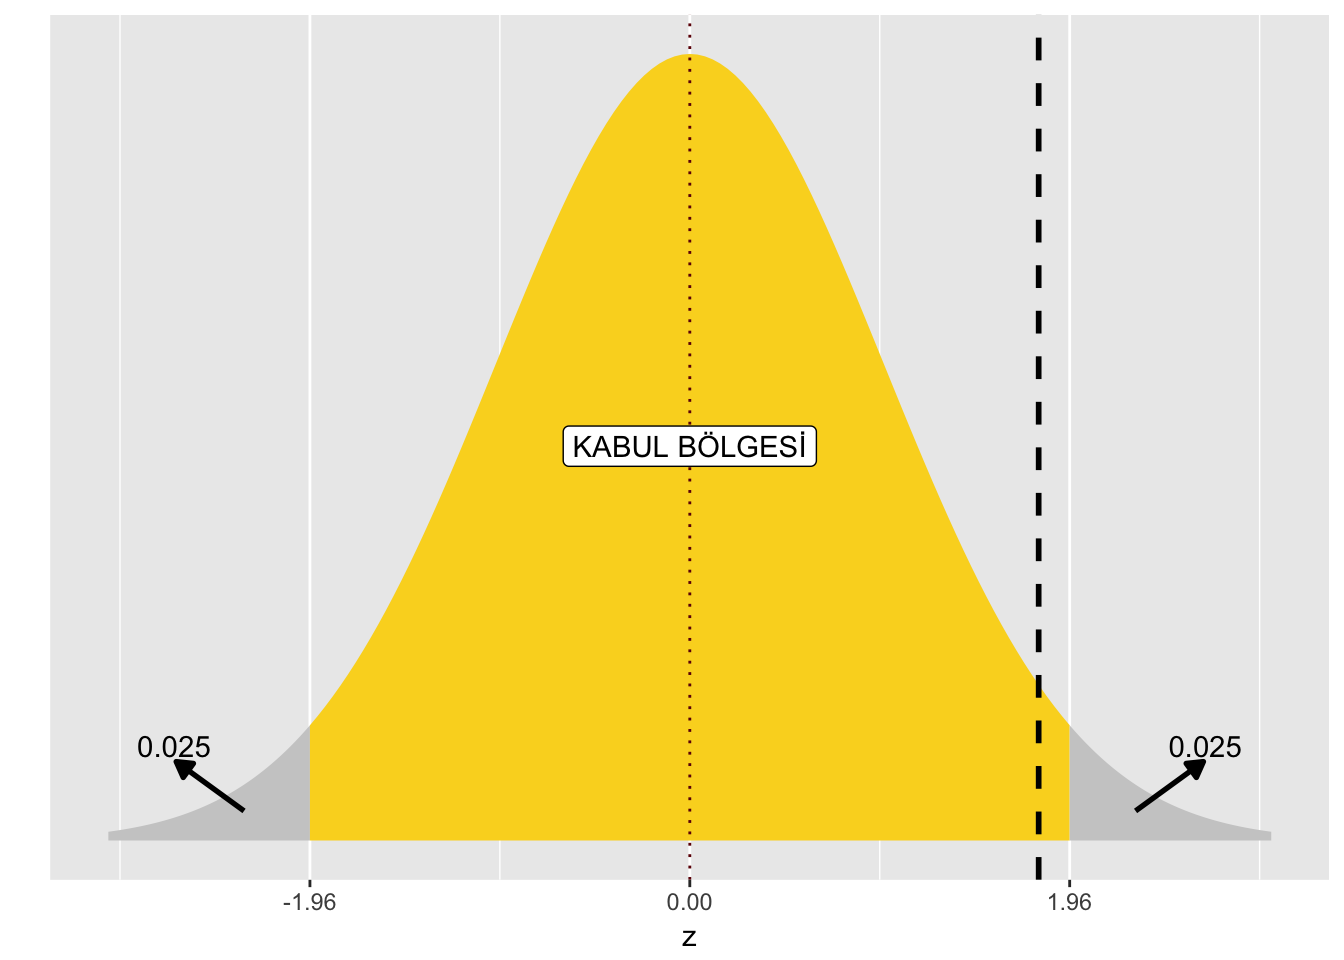
\includegraphics{03-Tests_files/figure-latex/unnamed-chunk-2-1.pdf}

Test istatistiği, taralı alan olan kabul bölgesine düşmediği için \(H_{0}\) boş hipotezini red edebilirsiniz. Yani, kutuları kozmetik ile aşırı doldurduğumuzdan makul bir şekilde şüphelenebiliriz.

\hypertarget{r-kodu}{%
\subsection{R-kodu}\label{r-kodu}}

\begin{Shaded}
\begin{Highlighting}[]
\NormalTok{mu0 }\OtherTok{\textless{}{-}} \FloatTok{4.0}
\NormalTok{n }\OtherTok{\textless{}{-}} \DecValTok{9}
\NormalTok{xbar }\OtherTok{\textless{}{-}} \FloatTok{4.6}
\NormalTok{sigma }\OtherTok{\textless{}{-}} \FloatTok{1.0}

\NormalTok{Z }\OtherTok{\textless{}{-}}\NormalTok{ (xbar }\SpecialCharTok{{-}}\NormalTok{ mu0) }\SpecialCharTok{/}\NormalTok{ (}\DecValTok{1} \SpecialCharTok{/} \FunctionTok{sqrt}\NormalTok{(n))}
\NormalTok{Z}
\end{Highlighting}
\end{Shaded}

\begin{verbatim}
## [1] 1.8
\end{verbatim}

İki yönlü hipotez testlerine ait p-değerini R kodu kullanarak da bulabiliriz. Yukarıdaki ilk grafiğe bakıldığında \(H_{0}\) boş hipotezini red edebilmek için Z değerinin mutlak değerce 1.8'den büyük olma olasılığı bulmamız gerekmektedir.

\begin{equation}
\begin{split}
P \left( |Z| \geq 1.8 \right) &= P(Z \geq 1.8) + P(Z \leq -1.8) \\
&= 1 - P(Z \leq 1.8) + P(Z \leq -1.8) \\
&= 1 - \phi(1.8) +\phi(-1.8)\\
\end{split}
\end{equation}

Burada \(\phi\) normal dağılımın birikimli (kümülatif) dağılım fonksiyonudur.

\begin{Shaded}
\begin{Highlighting}[]
\DecValTok{1} \SpecialCharTok{{-}} \FunctionTok{pnorm}\NormalTok{(}\FloatTok{1.8}\NormalTok{, }\AttributeTok{mean=}\DecValTok{0}\NormalTok{, }\AttributeTok{sd=}\DecValTok{1}\NormalTok{) }\SpecialCharTok{+} \FunctionTok{pnorm}\NormalTok{(}\SpecialCharTok{{-}}\FloatTok{1.8}\NormalTok{, }\AttributeTok{mean=}\DecValTok{0}\NormalTok{, }\AttributeTok{sd=}\DecValTok{1}\NormalTok{)}
\end{Highlighting}
\end{Shaded}

\begin{verbatim}
## [1] 0.07186064
\end{verbatim}

O halde p-değeri 0.07186064'dir. Bu p-değeri, belirlediğimiz anlamlılık düzeyi \(\alpha = 0.05\)'ten büyük olduğu için \(H_{0}\) boş hipotezini red edemezsiniz.

\hypertarget{test-2--}{%
\section{Test 2 -}\label{test-2--}}

\hypertarget{test-3--}{%
\section{Test 3 -}\label{test-3--}}

\hypertarget{test-4--}{%
\section{Test 4 -}\label{test-4--}}

  \bibliography{book.bib}

\end{document}
